% !TEX encoding = UTF-8
% !TEX TS-program = pdflatex
% !TEX root = ../tesi.tex
% !TEX spellcheck = it-IT

%**************************************************************
%\chapter{Analisi dei requisiti}
%\label{cap:analisi-requisiti}
%**************************************************************
%
%\intro{Breve introduzione al capitolo}\\
%
%\section{Casi d'uso}
%
%Per lo studio dei casi di utilizzo del prodotto sono stati creati dei diagrammi.
%I diagrammi dei casi d'uso (in inglese \emph{Use Case Diagram}) sono diagrammi di tipo uml dedicati alla descrizione delle funzioni o servizi offerti da un sistema, così come sono percepiti e utilizzati dagli attori che interagiscono col sistema stesso.
%Essendo il progetto finalizzato alla creazione di un tool per l'automazione di un processo, le interazioni da parte dell'utilizzatore devono essere ovviamente ridotte allo stretto necessario. Per questo motivo i diagrammi d'uso risultano semplici e in numero ridotto.
%
%\begin{figure}[!h] 
    %\centering 
    %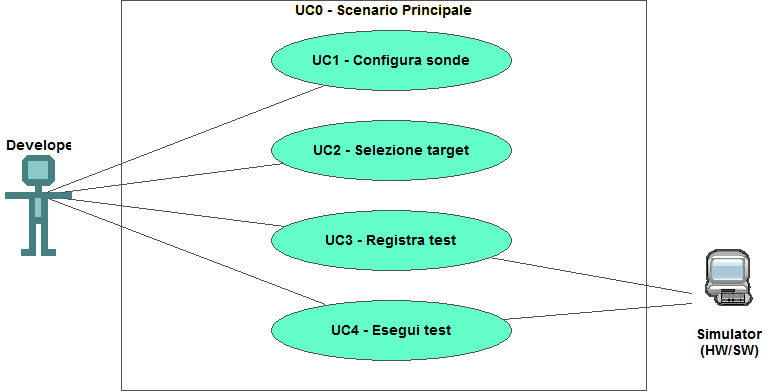
\includegraphics[width=0.9\columnwidth]{usecase/scenario-principale} 
    %\caption{Use Case - UC0: Scenario principale}
%\end{figure}
%
%\begin{usecase}{0}{Scenario principale}
%\usecaseactors{Sviluppatore applicativi}
%\usecasepre{Lo sviluppatore è entrato nel plug-in di simulazione all'interno dell'IDE}
%\usecasedesc{La finestra di simulazione mette a disposizione i comandi per configurare, registrare o eseguire un test}
%\usecasepost{Il sistema è pronto per permettere una nuova interazione}
%\label{uc:scenario-principale}
%\end{usecase}
%
%\section{Tracciamento dei requisiti}
%
%Da un'attenta analisi dei requisiti e degli use case effettuata sul progetto è stata stilata la tabella che traccia i requisiti in rapporto agli use case.\\
%Sono stati individuati diversi tipi di requisiti e si è quindi fatto utilizzo di un codice identificativo per distinguerli.\\
%Il codice dei requisiti è così strutturato R(F/Q/V)(N/D/O) dove:
%\begin{enumerate}
	%\item[R =] requisito
    %\item[F =] funzionale
    %\item[Q =] qualitativo
    %\item[V =] di vincolo
    %\item[N =] obbligatorio (necessario)
    %\item[D =] desiderabile
    %\item[Z =] opzionale
%\end{enumerate}
%Nelle tabelle \ref{tab:requisiti-funzionali}, \ref{tab:requisiti-qualitativi} e \ref{tab:requisiti-vincolo} sono riassunti i requisiti e il loro tracciamento con gli use case delineati in fase di analisi.
%
%\newpage
%
%\begin{table}%
%\caption{Tabella del tracciamento dei requisti funzionali}
%\label{tab:requisiti-funzionali}
%\begin{tabularx}{\textwidth}{lXl}
%\hline\hline
%\textbf{Requisito} & \textbf{Descrizione} & \textbf{Use Case}\\
%\hline
%RFN-1     & L'interfaccia permette di configurare il tipo di sonde del test & UC1 \\
%\hline
%\end{tabularx}
%\end{table}%
%
%\begin{table}%
%\caption{Tabella del tracciamento dei requisiti qualitativi}
%\label{tab:requisiti-qualitativi}
%\begin{tabularx}{\textwidth}{lXl}
%\hline\hline
%\textbf{Requisito} & \textbf{Descrizione} & \textbf{Use Case}\\
%\hline
%RQD-1    & Le prestazioni del simulatore hardware deve garantire la giusta esecuzione dei test e non la generazione di falsi negativi & - \\
%\hline
%\end{tabularx}
%\end{table}%
%
%\begin{table}%
%\caption{Tabella del tracciamento dei requisiti di vincolo}
%\label{tab:requisiti-vincolo}
%\begin{tabularx}{\textwidth}{lXl}
%\hline\hline
%\textbf{Requisito} & \textbf{Descrizione} & \textbf{Use Case}\\
%\hline
%RVO-1    & La libreria per l'esecuzione dei test automatici deve essere riutilizzabile & - \\
%\hline
%\end{tabularx}
%\end{table}%
%**************************************************************
\chapter{Accenni al funzionamento di Alfresco}
\label{cap:architettura}
%**************************************************************

\intro{In questo capitolo sarà esposto come creare un modulo e accenni all'architettura di Alfresco}\\

%**************************************************************
\section{architettura di Alfresco}
\section{Gestione dei moduli}
\subsection{creazione}
Bisogna innanzitutto rispondere ai prerequisiti descritti in  \href{http://docs.alfresco.com/sdk2.1/concepts/alfresco-sdk-installing-prerequisite-software.html}{questa pagina}.
Fatto questo il progetto può essere importato in un IDE, ad esempio per Eclipse in \href{http://docs.alfresco.com/community/tasks/alfresco-sdk-rad-eclipse-import-projects.html}{questo sito}
Le cartelle su cui andremo a sviluppare saranno la repo-amp e la share-amp. La share-amp verrà utilizzata per sviluppare l’interfaccia grafica del modulo mentre la parte di repo-amp  per lo sviluppo del “back-end”, le altre folder create servono per replicare l’ambiente di Alfresco in fase di esecuzione del modulo, e quindi non ha senso lavorare su di esse.
è necessario installare il driver jdbc se si intende  lavorare nell’SDK interagendo con database terzi, e dato che non è incluso nell'SDK anche se presente nell'ambiente finale, va incluso seguendo quanto detto in  \href{https://community.alfresco.com/thread/213317-sdk-21-including-third-party-jar-libraries}{questo luogo} . 
Una volta fatto questo, bisogna aprire nell’IDE o anche a mano all’indirizzo, partendo dalla cartella di installazione (sono riportati gli indirizzi utilizzando i nomi dell’esempio sopra citato: \texttt{/ alfresco-extension / acme-cms-poc / acme-cms-poc-share-amp / src / main / amp / config / alfresco / web-extension / site-webscripts / com / example / pages}
 (questo porta a dove è situata la pagina dimostrativa). È sufficiente fermarsi due o tre livelli sopra se l’intenzione è quella di mettere la gerarchia per una pagina custom (come fatto in questo progetto).
Una pagina fatta in alfresco share è composta da tre file, per semplicità prendiamo in considerazione la pagina di esempio già fornita:
un file .xml, che descrive i dati essenziali della pagina:
\begin{lstlisting}[language=XML]
<webscript>
    <shortname>Simple Page</shortname>
    <description>Simple page definition</description>
    <family>Share</family>
    <authentication>user</authentication>
    <url>/simple-page</url>
</webscript>
\end{lstlisting}
molto importanti sono il tag authentication, che specifica il livello di autenticazione necessario per accedere alla pagina, e il tag url, dal momento che definisce l’indirizzo della pagina, che sarà \texttt{<ip>:port/share/page/hdp/ws<url>} (hdp genera la pagina con header e footer, dp la pagina grezza).
Vi è poi il file .html che si comporta proprio come il body di una pagina html.
Vi è infine un file .js, che serve per applicare delle modifiche via json al model.
Quanto detto è sufficiente per creare una pagina che non necessiti di interazioni con java.

Per quanto riguarda una pagina che invece fa uso delle api di Alfresco il procedimento è più complicato: la pagina che verrà mostrata all’utente è collocata nella cartella \texttt{alfresco-extension /acme-cms-poc /acme-cms-poc-repo / amp / src / main / amp / config / alfresco / extension /templates / webscripts}.
La pagina generata è situata all’indirizzo \texttt{<ip>:<porta>/alfresco/service<url>}.
E’ inoltre necessario creare un bean che fa da collegamento tra il codice java, situato in \texttt{alfresco-extension / acme-cms-poc / acme-cms-poc-repo-amp / src / main / java / <package>}, e la pagina che verrà generata. Per farlo seguire quanto descritto in \href{http://docs.alfresco.com/community/tasks/bean-config.html}{questo sito}.

\subsection{Manutenzione}
Nel momento in cui si vorrà ad andare a modificare un modulo per evenienze riguardanti aspetti grafici o logici indiretti, bisognerà aprire il modulo con un IDE a piacere, e applicare le modifiche desiderate sui file. Il risultato delle modifiche effettuate è visionabile lanciando il comando \texttt{./run.sh} una volta posizionti all’interno della folder del modulo su linux, \texttt{run.bat} su windows, in alternativa al comando \texttt{mvn install -Prun}  o  \texttt{mvn clean install -Prun}, se è necessario anche svuotare la cache; avviato il server basterà
aprire il browser e digitare l’url : \texttt{<ip>:8080/share/page}.
Per quanto riguarda l’importazione dei moduli nell'ambiente di Alfresco vero e proprio, si dovrà lanciare il comando \texttt{mvn clean install} all'interno sempre del folder del modulo e all’interno della cartella target delle rispettive cartelle repo-amp e share-amp si creeranno un repo-amp file e uno share-amp file. Questi dovranno essere inseriti rispettivamente nelle cartelle amps e amps\_share nell'ambiente dell'Alfresco di produzione.
Per installare il modulo  è necessario lanciare il file \texttt{alfresco-community/bin/apply\_amps.bat}, oppure lanciandolo tramite il flag \texttt{-force} se si ha già un modulo con lo stesso nome che si vuole sovrascrivere.
Attenzione
L’ installazione dei moduli comporta un deploy che sovrascriverà il contenuto delle cartelle
\texttt{tomcat/webapps/share} e \texttt{tomcat/webapps/alfresco}. Di conseguenza nel momento in cui si è andati ad effettuare delle estensioni direttamente all’interno di queste cartelle il contenuto andrà perso. Quindi prima di effettuare questa operazione è necessario fare il backup delle cartelle indicate precedentemente.

\emph{Per comodità d’ora in poi il nome del progetto sarà indicato come AIOProject}.